%%%%%%%%%%%%%%%%%%%%%%%%%%%%%%%%%%%%%%%%%%%%%%%%%%%%%%%%%%%%%%%%%%%%%
% Pre�mbulo
%%%%%%%%%%%%%%%%%%%%%%%%%%%%%%%%%%%%%%%%%%%%%%%%%%%%%%%%%%%%%%%%%%%%%
\documentclass[a4paper,12pt]{imethesis}
\usepackage{indentfirst}
\usepackage[latin1]{inputenc}
\usepackage[portuges]{babel}
\usepackage[T1]{fontenc}                            % Fontes acentuados
%\usepackage[brazil]{babel}                          % L�ngua Portuguesa
%\usepackage{wrapfig}
%\usepackage{subfig}
\usepackage{nomencl} % Lista de Abreviaturas


%\usepackage[brazil]{babel}
\usepackage[usenames]{color}
\usepackage{graphicx}
%\usepackage{graphicx,color}
%\usepackage{graphicx}
%\usepackage[section]{placeins}

%\usepackage{algorithm}
%\usepackage{algorithmic}
\usepackage{float}      
%\usepackage{fancyvrb}
%\usepackage{boxit}
%\usepackage{listings}

\setlength{\hoffset}{-1cm}
\setlength{\voffset}{-2cm}
\setlength{\textheight}{23cm}
\setlength{\textwidth}{16cm}





%\usepackage{amsfonts}
\usepackage{amsthm,amsfonts}
\usepackage{amssymb}
\usepackage{epsfig}
%\usepackage{supertabular}
%\usepackage{epsf} %adicionado
\usepackage[authoryear,round]{natbib}
%\usepackage{latexsym}
%\usepackage[center]{caption}% usa um pacote para centralizar os captions das figuras e tabelas.
\usepackage{arydshln} %para fazer linhas pontilhadas na matriz
\sloppy

\usepackage{multirow}
% Define ambiente para Lema (definir outros sfc)
\newtheorem{teorema}{Teorema}[chapter]
\newtheorem{lema}{Lema}[chapter]
\newtheorem{definicao}{Defini��o}[chapter]

%\makeatletter
%\renewcommand{\@tocrmarg}{5em}
%\makeatother
\makenomenclature
%\makeglossary


%%%%%%%%%%%%%%%%%%%%%%%%%%%%%%%%%%%%%%%%%%%%%%%%%%%%%%%%%%%%%%%%%%%%%
% Fim do pre�mbulo
%%%%%%%%%%%%%%%%%%%%%%%%%%%%%%%%%%%%%%%%%%%%%%%%%%%%%%%%%%%%%%%%%%%%%

%%%%%%%%%%%%%%%%%%%%%%%%%%%%%%%%%%%%%%%%%%%%%%%%%%%%%%%%%%%%%%%%%%%%%
% Separa��o de s�labas
%%%%%%%%%%%%%%%%%%%%%%%%%%%%%%%%%%%%%%%%%%%%%%%%%%%%%%%%%%%%%%%%%%%%%
\hyphenation{}

%%%%%%%%%%%%%%%%%%%%%%%%%%%%%%%%%%%%%%%%%%%%%%%%%%%%%%%%%%%%%%%%%%%%%
% FIM DA SEPARA��O DE S�LABAS EXTRAS
%%%%%%%%%%%%%%%%%%%%%%%%%%%%%%%%%%%%%%%%%%%%%%%%%%%%%%%%%%%%%%%%%%%%%


%%%%%%%%%%%%%%%%%%%%%%%%%%%%%%%%%%%%%%%%%%%%%%%%%%%%%%%%%%%%%%%%%%%%%
% INICIO DO DOCUMENTO

%%%%%%%%%%%%%%%%%%%%%%%%%%%%%%%%%%%%%%%%%%%%%%%%%%%%%%%%%%%%%%%%%%%%%



\begin{document}

\begin{titlepage}

\begin{center}
\large{MINIST�RIO DA DEFESA} \\
\large{EX�RCITO BRASILEIRO} \\
\large{DEPARTAMENTO DE CIʊNCIA E TECNOLOGIA}\\
\large{IME - INSTITUTO MILITAR DE ENGENHARIA} \\
\large{CURSO DE GRADUA��O EM ENGENHARIA DA COMPUTA��O} \\
\vspace{5 cm}
\large{CAMILA ANTONACCIO WANOUS} \\
\large{JO�O LUIZ DO PRADO NETO} \\
\large{THIAGO DE PAULA VASCONCELOS} \\
\vspace{5 cm}
\large{CONECTIVIDADE ALG�BRICA E SEUS AUTOVETORES NA CLASSE DAS �RVORES}\\
\vspace{5 cm}
Rio de Janeiro\\
2013
\end{center}

\end{titlepage}


\def\figurename{\nomefigura\hspace{-0.8ex}}
\def\tablename{\nometabela\hspace{-0.7ex}}

%%%%%%%%%%%%%%%%%%%%%%%%%%%%%%%%%%%%%%%%%%%%%%%%%%%%%%%%%%%%%%%%%%%%%%%%%%%%%%%%%%%
%Folha de rosto
%%%%%%%%%%%%%%%%%%%%%%%%%%%%%%%%%%%%%%%%%%%%%%%%%%%%%%%%%%%%%%%%%%%%%%%%%%%%%%%%%%%
\university{Instituto Militar de Engenharia}
\title{Conectividade Alg�brica e seus Autovetores na Classe das �rvores}
\author{Camila Antonaccio Wanous}
\abrevauthor{Wanous, c.} 
%\patente{}
\cipcode{Z34r}
\date{Primeiro de Outubro 2013}
\cityear{Rio de Janeiro}{2013}

\chair{Claudia Marcela Justel - D.Sc.} {do IME}

\memberone{Maj Julio Cesar Duarte - D.Sc.}{do IME}
\membertwo{Prof. Maria Claudia Reis Cavalcanti - D.Sc.}{do IME}
 
\numberofmembers{3}

\thesisapp{Inicia��o � Pesquisa apresentada ao Curso de Gradua��o
em Engenharia de Computa��o do Instituto Militar de
Engenharia.} 

\maketitle

\begin{frontmatter}

\makecredits% \mbox{} %\clearpage
%---------------------------------------
%\copyrightpage
%---------------------------------------
\approvalpage %\mbox{} %\clearpage
%%%%%%%%%%%%%%%%%%%%%%%%%%%%%%%%%%%%%%%%%%%%%%%%%%%%%%%%%%%%%%%%%%%%%%%%%%%%%%%%%%%
%Dedicat�ria
\begin{dedicatoria}
  A nossos familiares e amigos, que indiretamente ajudaram no desenvolvimento do trabalho.
\end{dedicatoria}

%%%%%%%%%%%%%%%%%%%%%%%%%%%%%%%%%%%%%%%%%%%%%%%%%%%%%%%%%%%%%%%%%%%%%%%%%%%%%%%%%%
%pagina de agradecimentos
%\input{agradecimentos.tex}

%\begin{epigrafe}

%Ep�grafe

%\vspace{0.5cm}
%\hspace{0.3cm} ``O impulso para descobrir segredos est� profundamente enraizado na natureza humana.''
%\vspace{0.5cm}
%\hspace{6.5cm}  John Chadwick                     
%\end{epigrafe}

\tableofcontents
\listoffigures  
\listoftables
\listofnicks
\renewcommand{\nomname}{Lista de Siglas}
\printnomenclature %lista de abrevia��es
%\printglossary %lista de abrevia��es

%resumo
%\chapter*{Resumo}

O objetivo deste trabalho é prever como um time de futebol de robôs irá se comportar baseado
somente nas posições e orientações de um conjunto discreto de amostras. Para isso, foram estudados
os métodos da ACO (Ant Colony Optimization), SA (Simulated Annealing), Algorítimo  Genético, Lógica Nebulosa
e Redes Neurais. A partir do estudo detalhado desse algoritmos definiu-se duas linhas principais de
ação para a solução do problema: uma baseada em Logica Nebulosa e a outra baseada em Redes Neurais. Após
um estudo mais aprofundado deseja-se implementar um processo de otimização em ambos os algorítimos para
que o resultado seja refinado.

%\pagebreak

\end{frontmatter}



\chapter*{Resumo}

O objetivo deste trabalho é prever como um time de futebol de robôs irá se comportar baseado
somente nas posições e orientações de um conjunto discreto de amostras. Para isso, foram estudados
os métodos da ACO (Ant Colony Optimization), SA (Simulated Annealing), Algorítimo  Genético, Lógica Nebulosa
e Redes Neurais. A partir do estudo detalhado desse algoritmos definiu-se duas linhas principais de
ação para a solução do problema: uma baseada em Logica Nebulosa e a outra baseada em Redes Neurais. Após
um estudo mais aprofundado deseja-se implementar um processo de otimização em ambos os algorítimos para
que o resultado seja refinado.
 

\chapter{Introdução}


Segundo a \textit{wikipedia}:
\textit{"Robotics is the branch of technology that deals with the design, construction,
operation, and application of robots,as well as computer systems for their control,
sensory feedback, and information processing"}. As influencias da robótica já
são visíveis na indústria moderna. Ela tem viabilizado o desenvolvimento de peças
precisas, assim como um controle maior do processo. O uso de robôs confere aos
processos industriais precisão e repetibilidade maior que as adquiridas caso
fosse empregado um humano. Isso, além de reduzir o custo de retrabalhos, permite
que os desenvolvedores se preocupem mais com o processo em si. Assim, o emprego
de robôs confere um amadurecimento dos processos industrias, bem como indiretamente
permite que a sociedade concentre esforços em cargos intelectuais.

Com efeito, o emprego desses sistemas robóticos deixou evidente a necessidade do
desenvolvimento de teorias relacionadas as sistemas autônomos. Esses sistemas podem
ser empregados para permitir que resgates sejam feitos de maneira eficiente. Isso
evitaria que o pessoal altamente especializado empregado atualmente corra risco de vida.

Entretanto, projetar robôs autônomos para trabalharem juntos não é uma tarefa trivial. Essa
tarefa se complica quando um robô não tem um modelo bem definido dos outros robôs que atuarão em
conjunto. Um domínio de aplicação que envolve essa problemática é o futebol de robôs.
Nesse domínio é comum a distribuição de papéis dinamicamente entre os membros de cada
time. Entretanto, um time não tem conhecimento dos papéis atribuídos aos robôs
do time oponente. O planejamento de um time pode ser aprimorado através de um modelo
aproximado desse time oponente, pois levará em consideração a maneira como o
time reagirá às diversas ações possíveis.

A seguir, descreve-se a história da competição de futebol de robôs.

\begin{figure}
  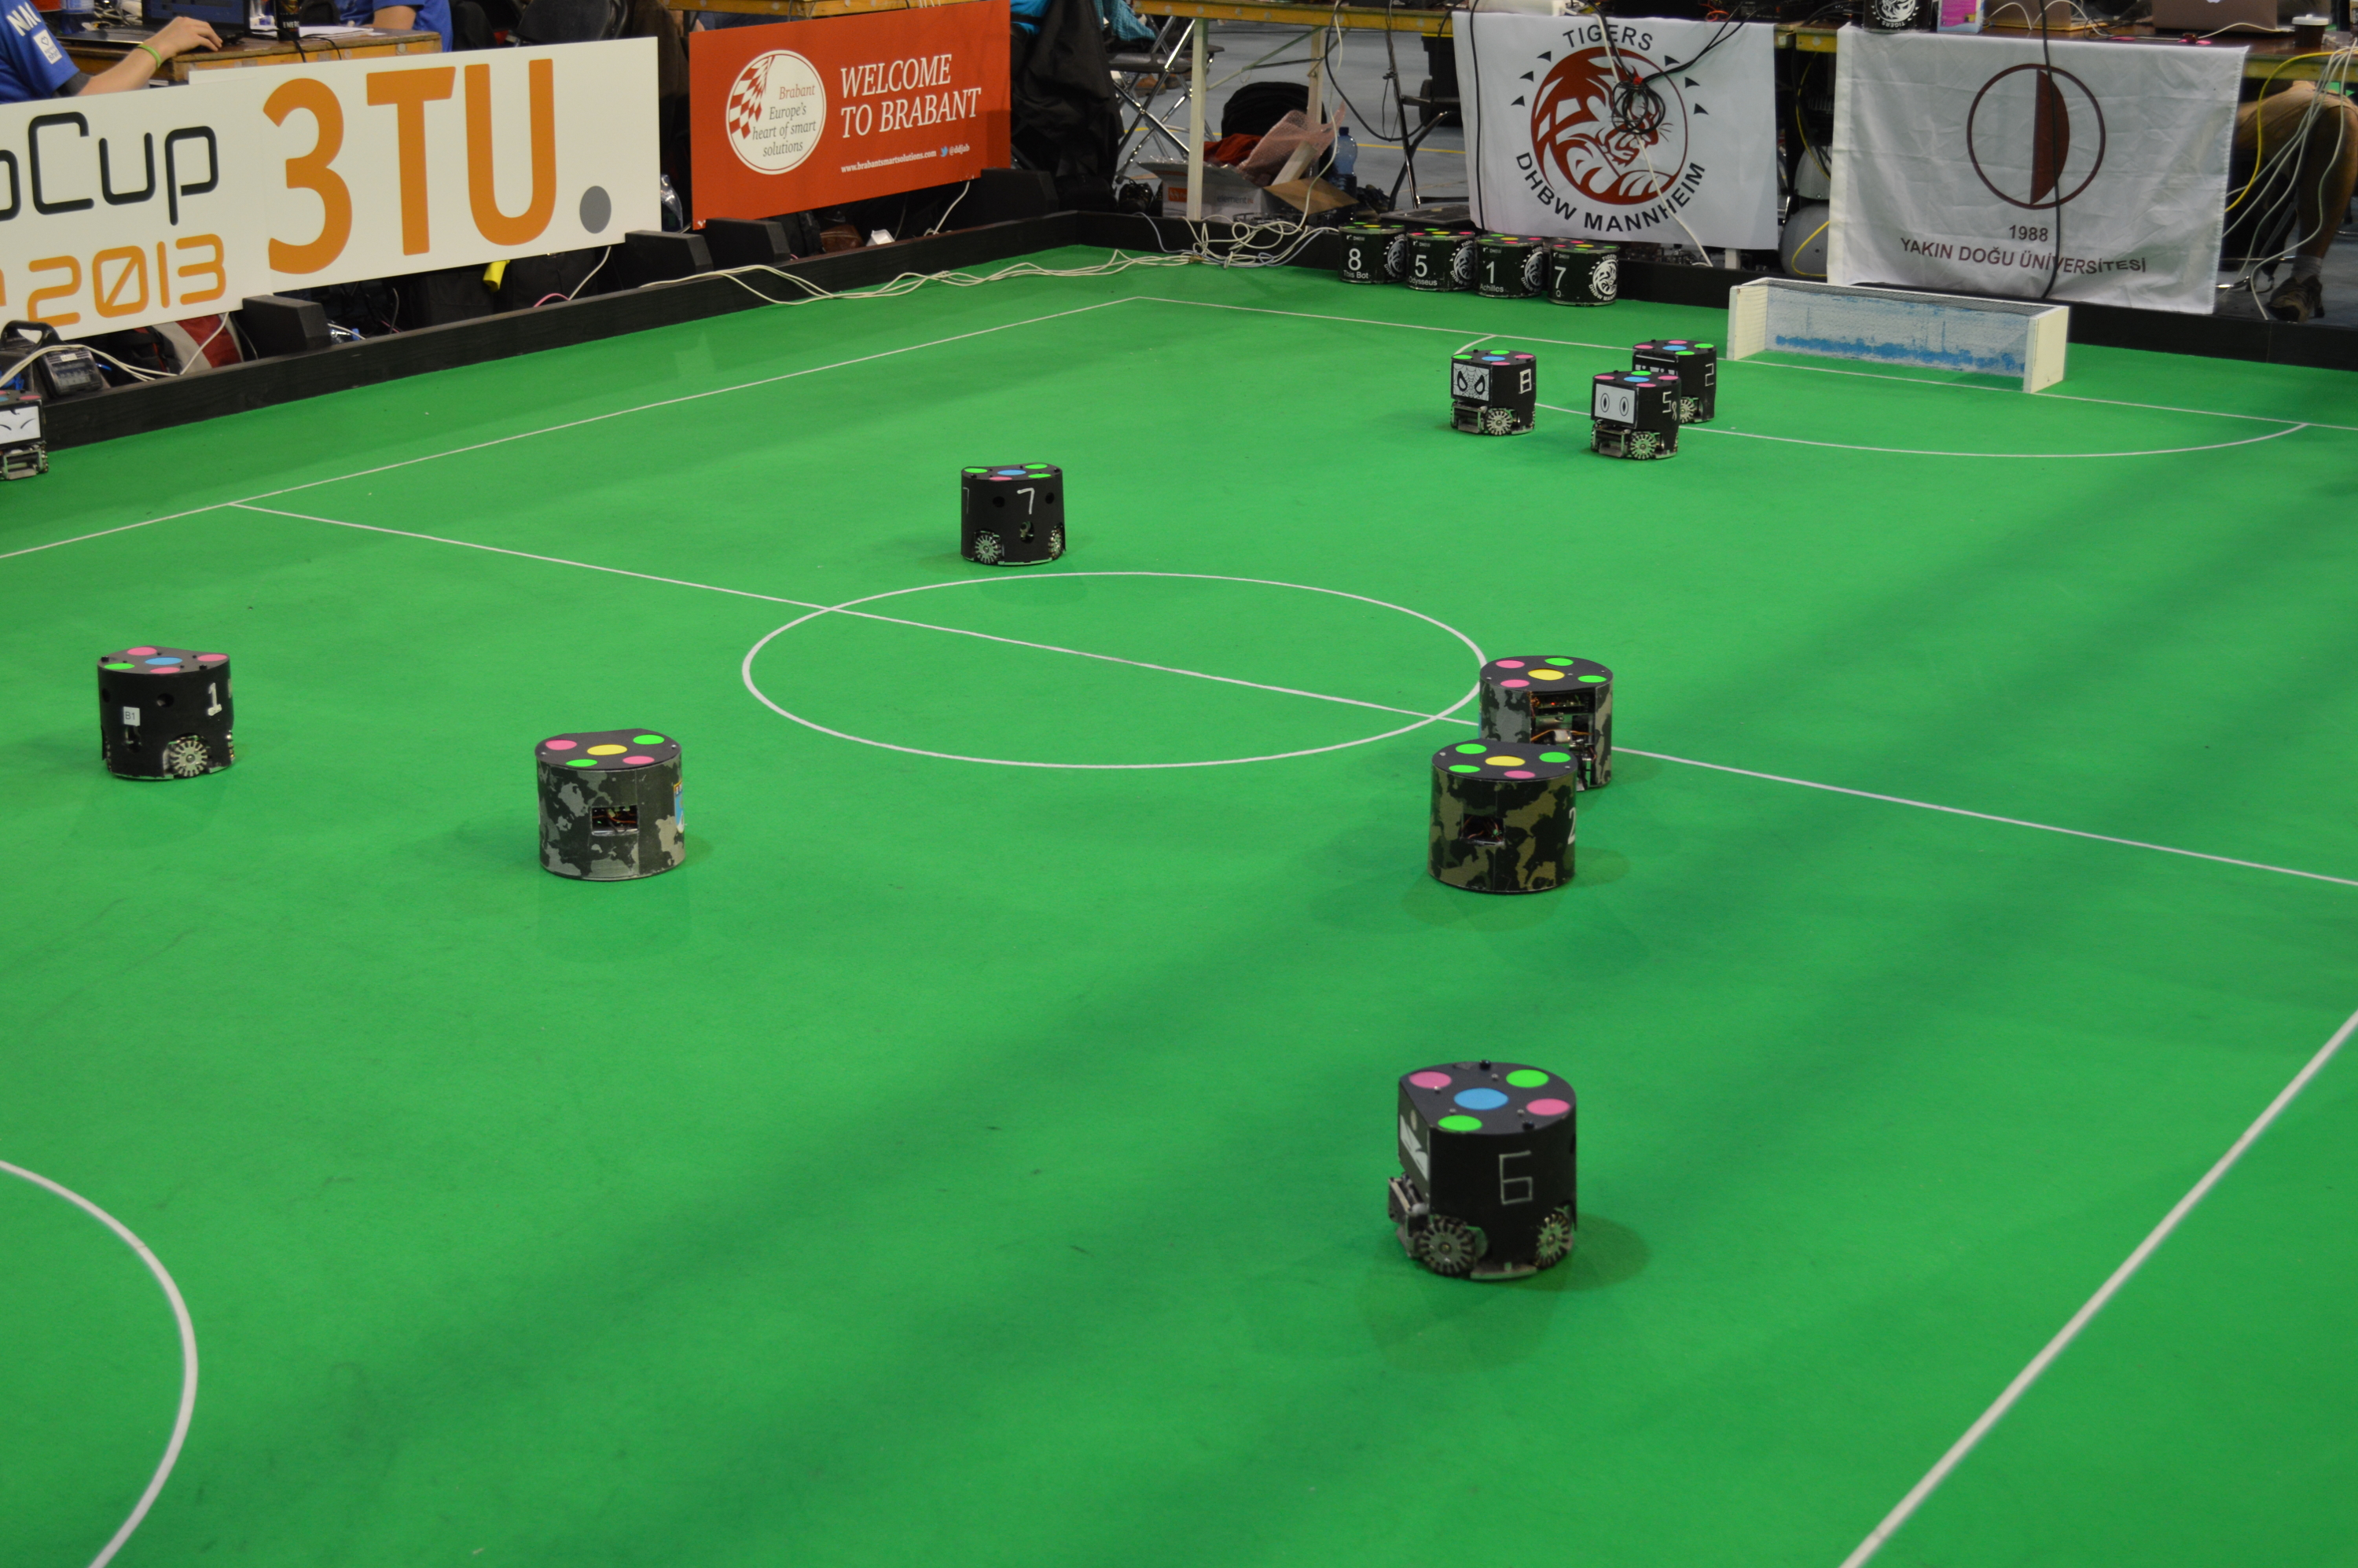
\includegraphics[width = \linewidth]{figuras/robocup2013}
  \caption{Imagem da SSL \textit{RoboCup} 2013 em Eindhoven, na Holanda}\label{fig:robocup2013}
\end{figure}

A ideia de robôs jogando futebol foi mencionada pela primeira vez pelo professor
Alan Mackworth (\textit{University of British Columbia}, Canadá) em um artigo intitulado
\textit{"On Seeing Robots"}, apresentado no \textit{Vision Interface 92} e posteriormente publicado em
um livro chamado \textit{Computer Vision: System, Theory and Applications}. Independentemente,
um grupo de pesquisadores japoneses organizou um \textit{Workshop} no \textit{Ground Challange
in Artificial Inteligence}, em Outubro de 1992, Tóquio, discutindo e propondo problemas que
representavam grandes desafios. Esse \textit{Workshop} os levou a sérias discussões sobre
usar um jogo de futebol para promover ciência e tecnologia. Estudos foram feitos para
analisar a viabilidade dessa ideia. Os resultados desses estudos mostram que
a ideia era viável, desejável e englobava diversas aplicações práticas. Em 1993, um
grupo de pesquisadores, incluindo Minoru Asada, Yasuo Kuniyoshi e Hiroaki Kitano,
lançaram uma competição de robótica chamada de Robot \textit{J-League} (fazendo uma analogia à
\textit{J-League}, nome da Liga Japonesa de Futebol Profissional). Em um mês, vários
pesquisadores já se pronunciavam dizendo que a iniciativa deveria ser estendida ao
âmbito internacional. Surgia então, a \textit{Robot World Cup Initiative} (RoboCup).

RoboCup é uma competição destinada a desenvolver os estudos na área de robótica e
Inteligência Artificial (IA) por meio de uma competição amigável. Além disso, ela tem
como objetivo, até 2050, desenvolver uma equipe de robôs humanoides totalmente
autônomos capazes de derrotar a equipe campeã mundial de futebol humano. A competição
possui várias modalidades. Neste trabalho, será analisada a \textit{Small Size Robot League} (SSL),
também conhecida como F180. De acordo com as regras da SSL, as equipes devem ser
compostas por 6 robôs, sendo um deles o goleiro, que deve ser
designado antes do início do jogo. Durante o jogo, nenhuma interferência humana é
permitida com o sistema de controle dos robôs. É fornecido aos times um sistema de
visão global e esses controlam seus robôs com máquinas próprias. O sistema de controle
dos robôs geralmente é externo e recebe os dados de um conjunto de duas câmeras
localizadas acima do campo. Esse sistema de controle processa os dados, determina qual comando deve ser executado por
cada robô e envia este comando através de ondas de rádio aos robôs. Embora seja
permitido que as equipes utilizem sistemas próprios de visão, a maioria das
<<<<<<< HEAD
equipes utiliza a visão centralizada. A figura~\ref{fig:robocup2013} mostra uma
imagem da SSL Robocup 2013, da qual o a ROBOIME (Equipe de Futebol de Robôs do
=======
equipes utiliza a visão centralizada. A figura~\ref{robocup2013} mostra uma
imagem da SSL Robocup 2013, da qual a RoboIME (Equipe de Futebol de Robôs do
>>>>>>> 2bbffc8258d22096146654d1423c9b3d9363efdb
Laboratório de Robótica do IME) participou.

\section{Motivação}

O futebol de robôs, problema padrão de investigação internacional, reúne grande parte
dos desafios presentes em problemas do mundo real a serem resolvidos em tempo real.
As soluções encontradas para o futebol de robôs podem ser estendidas, possibilitando
o uso da robótica em locais de difícil acesso para humanos, ambientes insalubres e
situações de risco de vida iminente.

Há diversas novas áreas de aplicação da robótica, tais como exploração espacial e submarina,
navegação em ambientes inóspitos e perigosos, serviço de assistência médica
e cirúrgica, além do setor de entretenimento. Essas áreas podem ser beneficiadas com o
desenvolvimento de sistemas
multi robôs. Nestes domínios de aplicação, sistemas de multi robôs deparam-se sempre
com tarefas muito difíceis de serem efetuadas por um único robô. Um time de robôs pode
prover redundância e contribuir cooperativamente para resolver o problema em questão.
Com efeito, eles podem resolver o problema de maneira mais confiável, mais rápida e
mais econômica, quando comparado com o desempenho de um único robô.

% TODO Incluir imagem do robô
%\begin{figure}
%  \includegraphics[width = \pagewidth]{}
%\end{figure}

Devido à grande complexidade do problema de interação com humanos, faz-se necessário
que os robôs sejam dotados de uma capacidade de aprendizado para facilitar a interação
desses com o mundo real. Isso é relevante tanto para aplicações industriais, quanto para
aplicações em resgates e militares. Isso diminui a necessidade de modelagem
exata dos ambientes em que os sistemas robóticos serão introduzidos e permite que
a adaptação a ambientes complexos seja realizada através da exposição destes sistemas
às possíveis situações de trabalho. Por meio da incorporação do sistema de
aprendizagem, situações não consideradas podem ser incorporadas ao algoritmo de
controle dos robôs dinamicamente. Isso permitiria que esses reagissem de maneira mais
eficiente em futuras situações semelhantes.

\section{Objetivo}

Este trabalho objetiva, através do processo de \textit{Mineração de Dados}, extrair
informação dos $logs$ (definido a seguir) de um jogo do futebol de robôs.
Isso tem o objetivo de permitir que agentes controláveis
possam reagir de maneira eficiente às ações dos agentes do time adversário, que não são controláveis.
A pesquisa se propõe a realizar esse aprendizado dos agentes adversários baseado em gravações
coletadas dos pacotes da \textit{SSL-Vision} e do \textit{Referee-Box} durante jogos, também conhecidas
como \textit{logs}, para posteriormente serem incorporados ao sistema de inteligência da
equipe de futebol de robôs do Laboratório de Robótica, denominada RoboIME.
% NOTE: acho que não é o caso disso:
%Se possível, deseja-se que essa modelagem/aprendizagem seja feita dinamicamente durante a partida da SSL.

\section{Justificativa}% TODO Maj Duarte colocou um certo nessa encestação

Um método concreto que possa prever o comportamento de agentes inteligentes de um jogo de
futebol de robôs permite com que seja possível prever o comportamento de um time adversário.
Com tal mecanismo é possível melhorar a Inteligência Artificial em uso pela RoboIME
para tomar decisões que levem a resultados melhores e, por consequência, ganhar mais partidas.
Outras equipes participantes da SSL já utilizam mecanismos de predição do adversário.
Portanto, é de grande importância desenvolver também tal mecanismo para acompanhar a evolução
das tecnologias envolvidas.

\section{Metodologia}

Para atingir os objetivos propostos, será seguida a seguinte metodologia:
Inicialmente o problema a ser investigado será definido formalmente,
utilizando definições e teorias apropriadas.

Posteriormente, a bibliografia é revisada e são evidenciados os métodos comumente
utilizados para a abordagem do problema mais geral de classificação, bem como são
analisados trabalhos aplicados especificamente à SSL.

A seguir, são analisadas as heurísticas levantadas durante a
revisão da bibliografia. Cada uma delas é descrita. Após descrição sumária
de cada heurística, são apresentados os respectivos exemplos de cada aplicação.

Então, são apresentadas abordagens envolvendo as heurísticas introduzidas
anteriormente. Cada abordagem relaciona, no mínimo, uma dessas heurísticas.
Ao final de cada seção, é apresentado uma metodologia a ser aplicada
na resolução do problema. Uma análise das características de cada abordagem
é feita ao final da descrição de cada abordagem.

<<<<<<< HEAD
A seguir, são descritos possíveis algoritmos para implementar essas abordagens.
Essas abodragens são analisadas.
=======
A seguir, são descritos possíveis algoritmos para implementar essas abordagens. Também são
desenvolvidas métricas para avaliar os algoritmos desenvolvidos.
>>>>>>> 2bbffc8258d22096146654d1423c9b3d9363efdb

% NOTE: não é bem verdade isso:
%Para validar os estudos desenvolvidos, o projeto de um software
%que analise os dados dos \textit{logs} disponíveis no site da SSL é apresentado.

\section{Estrutura do Trabalho}

No capítulo~\ref{cap:def_problema}, o problema a ser resolvido é definido formalmente.

No capítulo~\ref{cap:rev_bibliografica}, a bibliografia é revisada.

No capítulo~\ref{cap:heuristicas}, são apresentados tutoriais relacionados às
heurísticas comumente utilizadas em problemas de classificação.

No capítulo~\ref{cap:anal_abordagens}, são descritas possíveis abordagens a serem
seguidas para resolução do problema.

No capítulo~\ref{cap:conclusao}, são apresentadas as principais conclusões atingidas.
 

\chapter{�rvores}
\section{Teoria dos Grafos}
Um \textbf{grafo} � uma estrutura $G=G(V,E)$, em que $V$ � um conjunto finito e n�o vazio cujos elementos s�o chamados de \textbf{v�rtices}, enquanto $E$ representa um conjunto de subconjuntos de pares de elementos de $V$, subconjuntos estes denominados \textbf{arestas}, neste trabalho iremos considerar que grafos n�o possuem la�os (arestas do tipo ($v,v$)), nem arestas repetidas.

Se $v$ � um v�rtice do grafo $G$, o \textbf{grau} de $v$, denotado por $d(v)$, � o n�mero de arestas que incidem em $v$, em que aresta incidente em $v$ � aquela que liga o v�rtice $v$ a outro v�rtice de $G$. Iremos denotar por $\Delta(G)$ o \textbf{grau m�ximo} em $G$, que � o grau do v�rtice de maior grau dentre os v�rtices de $G$, e por $\delta(G)$  o \textbf{grau m�nimo} em $G$, que � o grau do v�rtice de menor grau dentre os v�rtices de $G$.

Uma sequ�ncia de v�rtices $v_1,~v_2,~\ldots,~v_k$, onde ($v_i,v_{i+1}$) $\epsilon~E(G)$ para $1\leq i\leq k-1$,  $k>1$, � dita um \textbf{passeio}, com os v�rtices $v_1$ e $v_k$ sendo as extremidades do passeio e o valor $k-1$ o tamanho do passeio. Se as arestas ($v_i,v_{i+1}$), para $1\leq i\leq k-1$, forem todas distintas dizemos que o passeio � uma trilha. Se, al�m disso, os v�rtices  $v_1,~v_2,~\ldots,~v_k$ forem distintos, a trilha se chama \textbf{caminho}. Um \textbf{ciclo} � um passeio fechado $v_1, ... v_k$, onde $v_1 = v_k$, $k$ maior ou igual a $4$ e $v_1,...v_{k-1}$ � um caminho. Dizemos que um grafo $G$ � \textbf{conexo} se partindo de cada v�rtice de $G$ existe um caminho para qualquer outro v�rtice do grafo, caso contr�rio o grafo � dito \textbf{desconexo}. Para os conceitos a seguir sejam $v$ e $w$ dois v�rtice do grafo $G$, a \textbf{dist�ncia} entre dois $v$ e $w$, denotada por $d(v,w)$ � o menor caminho entre dois v�rtices.  A \textbf{excentricidade} do v�rtice $v$ � $e(v)=max_{w \epsilon V(G)}d_G(v,w)$. A maior dessas dist�ncias � chamada \textbf{di�metro} do grafo. O \textbf{centro} do grafo $G$ � o subconjunto de $V(G)$ formado pelos v�rtices de excentricidade m�nima.

Seguiremos com o conceito de �rvore. Uma \textbf{�rvore} � um grafo conexo $G$ que n�o possui ciclos. Isso nos leva as seguintes propriedades: um grafo $G$, com $n$ v�rtices e $m$ arestas � uma �rvore se, somente se, $m=n-1$ e $G$ � conexo, e um grafo $G$, com $n$ v�rtices e $m$ arestas � uma �rvore se, somente se, $G$ n�o possui ciclos e $m=n-1$.

\section{Teoria Espectral dos Grafos}
A \textbf{teoria espectral dos grafos} � o ramo da teoria dos grafos que se preocupa em determinar propriedades dos grafos por meio de suas representa��es matriciais e de seus respectivos espectros. Iremos ter por foco a matriz laplaciana do grafo.

Para definirmos a matriz laplaciana precisaremos definir a matriz de adjac�ncia e a matriz diagonal dos graus primeiro.

Seja $G = G(V,E)$ um grafo com v�rtices $v_1,~v_2,\ldots, ~v_n$. A \textbf{matriz de adjac�ncia} do grafo $G$, ou simplesmente matriz de adjac�ncia de $G$, � uma matriz quadrada cuja ordem � o n�mero de v�rtices de $G$. Se $G = G(V,E)$ � um grafo com v�rtices $v_1,~v_2,\ldots, ~v_n$, a matriz de adjac�ncia de $G$ � denotada por $A(G)$ e definida como a matriz quadrada de ordem $n$, $A(G)=(a_{ij})_{nxm}$, em que os $a_{ij}$ s�o dados por:

\begin{displaymath}
a_i_j = \left\{ \begin{array}{ll}
1, & \textrm{se~$\{v_i,v_j\}~\epsilon ~ E$;}\\
0, & \textrm{caso contr\'ario.}
\end{array} \right.
\end{displaymath}

Para definir a matriz diagonal dos graus consideremos $G = G(V,E)$ um grafo com v�rtices $v_1,~v_2,\ldots, ~v_n$. A \textbf{matriz diagonal dos graus} dos v�rtices de
$G$ � denotada por $D(G)$ e definida como a matriz quadrada $D(G)=(d_{ij})_{nXm}$, em que $d_{ij}$ � dado por:

\begin{displaymath}
d_i_j = \left\{ \begin{array}{ll}
d(v_i), & \textrm{se~$i=j$;}\\
0, & \textrm{caso contr\' ario.}
\end{array} \right.
\end{displaymath}

Observemos que, por ser uma matriz diagonal, a matriz � sim�trica.

Conhecendo estes conceitos podemos prosseguir com a defini��o de matriz laplaciana. Seja $ = G(V,E)$ um grafo. A \textbf{matriz laplaciana} de $G$ � denotada por $L(G)$ e definida como a matriz quadrada $L(G)=A(G)-D(G)$. Observemos que como a matriz laplaciana � a diferen�a entre duas matrizes sim�tricas ela tamb�m � sim�trica.

Conhecendo a defini��o de matriz laplaciana podemos definir a conectividade alg�brica, que � um autovalor da matriz laplaciana e est� associado a qu�o conexo � o grafo, e o vetor de Fiedler.

Sejam $G$ um grafo e $\mu_1 \ge \ldots \ge \mu_n$ os autovalores da matriz laplaciana $L(G)$. A \textbf{conectividade alg�brica} do grafo $G$, denotada por $a(G)$, � $\mu_n_-_1$. J� o autovalor $\mu_1$ � chamado de \textbf{�ndice do laplaciano} de $G$. Definiremos ainda o \textbf{raio espectral} do grafo, denotado por $\rho(G)$, como sendo $\rho(G)=max|\lambda_i|$, $i=1,~2,\ldots,~n$. O autovetor associado a conectividade alg�brica � chamado de \textbf{vetor de Fiedler}.

O vetor de Fiedler ser� usado para classificar as �rvores em �rvores de tipo $I$ e de tipo $II$. Iremos discutir sobres estas �rvores na pr�xima se��o.

\section{�rvores de Tipo $I$ e de Tipo $II$}

Nesta se��o explicaremos como classificar as �rvores a partir do vetor de Fiedler em �rvores de tipo $I$ e em �rvores de tipo $II$. Iniciaremos definindo quando uma �rvore � de tipo $I$.

\begin{itemize}

\item Uma �rvore $T$ � dita ser de tipo $I$ se:

\begin{enumerate}

\item existe alguma entrada de $y$ igual a $0$, nesse caso o conjuntos de v�rtices do subgrafo induzido por este que correspondem aos zeros est�o conectados.

\item existe somente um v�rtice $k$ tal que $y_k=0$ e $k$ � adjacente a algum v�rtice $m$ (pode ser mais do que um v�rtice $m$, com $y_m \neq 0$. As entradas de $y$ podem ser crescentes, decrescentes ou iguais a $0$ ao longo de qualquer caminho de $T$ que comece em $k$.

Seguiremos definindo quando uma �rvore � de tipo $II$.

\end{enumerate}

\item Uma �rvore $T$ � dita ser de tipo $II$ se:

\begin{enumerate}

\item nenhuma entrada de $y$ � $0$.

\item existe somente um par de v�rtices adjacentes $i$ e $j$, tais que $y_i>0$ e $y_j<0$, al�m disso as entradas de $y$ s�o crescentes ao longo do caminho em $T$ que come�a em $i$ e n�o cont�m $j$, enquanto as entradas de $y$ para o caminho que come�a $j$ e n�o cont�m $i$ s�o decrescentes.

\end{enumerate}

\end{itemize}

Isto �, as �rvores de tipo $I$ s�o tais que se um v�rtice $k$ corresponde a $y_k=0$, ent�o ele separa o grafo em dois subgrafos, um subgrafo corresponde �s entradas nulas e outro �s entradas n�o nulas. J� as �rvores de tipo $II$ possuem conceito mais simples, basta que nenhuma das entradas do vetor de Fiedler seja $0$. Como exemplo, apresentamos uma �rvore de tipo $I$ na Figura 2.1.

\begin{figure}[H] %h,t,b,p,H%
\centering
\includegraphics[width=2cm]{arvore}
\caption{�rvore de tipo $I$.}
%width mexe no tamanho e angle na rotação%
\label{fig:genrang}
\end{figure}

A �rvore da Figura 2.1 possui conectividade alg�brica $a(T)=0,2678$ e  vetor de Fiedler igual a [$0,440;~ 0,440;~ 0,3251;~ 	0;~ 0;~ -0,3251;~ -0.440;~ -0,440$]. Observe que, de fato, somente um v�rtice correspondente a $0$, o v�rtice $4$, est� ligado � v�rtices correspondentes a entradas n�o-nulas, e ainda, partindo do v�rtice $4$ podemos escolher um caminho de entradas crescentes, decrescentes ou identicamente nulas.

Como exemplo de �rvore de tipo $II$, apresentamos a �rvore de $11$ v�rtices da Figura 2.2.

\begin{figure}[H] %h,t,b,p,H%
\centering
\includegraphics[width=7.5cm]{arvoretipoII}
\caption{�rvore de tipo $II$.}
%width mexe no tamanho e angle na rotação%
\label{fig:genrang}
\end{figure}

A �rvore da Figura 2.2, de conectividade alg�brica $0.42972$ e vetor de Fiedler igual a [$0,4502;~ -0,1446;~ -0,1446;~ -0,1446;~ -0,1446;~ -0,1446;~ -0,1446;~ -0,1446;~ -0,1446;$ $0,7894;~ -0,08249$]. Observe que, de fato, n�o h� v�rtices correspondetes a $0$, e ainda, s� h� uma aresta que une um v�rtice correspondente a um valor positivo a um v�rtice correspondente a um valor negativos, aresta $(v_1,v_{11})$.

\chapter{Ferramentas de Banco de Dados}

\section{Banco de Dados Relacional}

\subsection{Introdu��o ao modelo relacional}
No modelo relacional a constru��o se baseia em rela��es, que s�o representadas por meio de tabelas. Uma rela��o consiste de um esquema e de uma inst�ncia. O esquema especifica o nome da rela��o e o nome e o dom�nio de cada coluna, tamb�m denominada atributo ou campo da rela��o. O dom�nio do atributo � referenciado no esquema por seu nome e serve para restringir os valores que este atributo pode assumir. O esquema de uma rela��o � inv�riavel ao longo do tempo, sendo modificado apenas por comandos espec�ficos. Um exemplo de esquema de rela��o �:

Estudante (e$\_$id: integer, nome: string, login: string, nota: real).

Neste caso est� sendo definida a rela��o de nome Estudantes, com atributos e$\_$id, nome, login e nota, cujos dom�nios s�o respectivamente integer, string, string e real.

A inst�ncia de uma rela��o � o conjunto de linhas, tamb�m denominadas tuplas ou registros, distintas entre si, que comp�em a rela��o em um dado momento. Ela � vari�vel, j� que o n�mero de tuplas e o conte�do de seus atributos podem variar ao longo do tempo. A inst�ncia de uma rela��o deve seguir sempre o seu respectivo esquema, respeitando o n�mero de atributos definidos, bem como os seus dom�nios. Esta restri��o, denominada restri��o de dom�nio, � muito importante. O modelo relacional somente considera rela��es que satisfa�am esta restri��o. Um exemplo de uma inst�ncia para o esquema estudantes � ilustrado na Tabela 3.1.

\begin{table}[H]
\centering
\begin{tabular}{|c|c|c|c|}
\hline
e\_$$id &	nome & login & nota\\
\hline
11403	& Camila & camila.atonaccio & 10\\ \hline
11422	& Jo�o Prado & joao.prado & 9,7\\ \hline
11442	& Thiago & thiago.vasconcelos & 9,8\\ \hline
\end{tabular}
\caption{Exemplo de inst�ncia para o esquema estudantes.}
\end{table}

O n�mero de tuplas que uma dada inst�ncia possui denomina-se cardinalidade da rela��o e o n�mero de atributos � o seu grau. A inst�ncia de rela��o da acima tem cardinalidade 3 e grau 5. Podemos notar que a cardinalidade � vari�vel, mas o grau n�o. Um banco de dados relacional � um conjunto de uma ou mais rela��es com nomes distintos. O esquema do banco de dados relacional � a cole��o dos esquemas de cada rela��o que comp�e o banco de dados.

\subsection{Ferramenta MySQL}
O MySQL � um sistema de gerenciamento open souce de bancos de dados relacional (armazena dados em tabelas separadas em vez de colocar todos os dados um s� local proporcionando velocidade e flexibilidade). O servidor de banco de dados MySQL � extremamente r�pido, confi�vel, e f�cil de usar.

O Servidor MySQL foi desenvolvido originalmente para lidar com bancos de dados muito grandes de maneira muito mais r�pida que as solu��es existentes e tem sido usado em ambientes de produ��o de alta demanda por diversos anos de maneira bem sucedida.

Essa ferramenta funciona nas mais diversas plataformas e pode ser escrito em C ou C++. Ele tem a capacidade de lidar com banco de dados enormes. Existe servidor com banco de dados MySQL que cont�m 50.000.000 (milh�es) de registros e sabemos de usu�rios que usam o MySQL com 60.000 (mil) tabelas e aproximadamente 5.000.000.000 (bilh�es) de linhas, al�m de possuir um sistema de aloca��o de mem�ria muito r�pido e baseado em processo (thread).

\section{Banco de Dados Orientado a grafos}

\subsection{Introdu��o ao modelo orientado a grafos}
Diferentemente do que acontece no modelo relacional, que armazena suas informa��es em linhas, colunas ou pares chaves, um banco de dados orientado a grafos armazena os dados em uma rede de n�s e arestas. Sendo as arestas respons�veis por representar o relacionamento e os n�s por representarem objetos.

Ao desenvolvermos uma aplica��o, geralmente nos deparamos com a situa��o de trabalharmos com o banco de dados relacional, realizando diversas queries complexas. Tais queries podem possuir essa complexidade devido ao fato de estarmos modelando dados que n�o s�o naturais ao paradigma relacional, em um banco relacional.

Um bom exemplo � uma aplica��o que tem por objetivo manter informa��es relativas a locais onde a pessoas morou e a viajou, como saber quais pessoas j� viveram em uma determinada cidade, ou saber quantas j� viajaram para uma determinada cidade.

Fazendo uso da modelagem por meio de um banco de dados relacional podemos chegar � estrutura de tabelas representadas em Tabela 3.2, Tabela 3.3, Tabela 3.4 e Tabela. 3.5.

\begin{table}[H]
\centering
\begin{tabular}{|c|c|}
\hline
id\_$$pessoa &	nome\\
\hline
1	& Jo�o Prado\\ \hline
2	& Camila\\ \hline
3	& Thiago\\ \hline
4	& Vin�cius\\ \hline
5	& Matheus\\ \hline
\end{tabular}
\caption{Pessoas.}
\end{table}

\begin{table}[H]
\centering
\begin{tabular}{|c|c|}
\hline
id\_$$cidade &	nome\\
\hline
1	& Aparecida\\ \hline
2	& S�o Jos� dos Campos\\ \hline
3	& S�o Paulo\\ \hline
4	& Rio de Janeiro\\ \hline
5	& Fortaleza\\ \hline
6	& Natal\\ \hline
\end{tabular}
\caption{Cidades.}
\end{table}

\begin{table}[H]
\centering
\begin{tabular}{|c|c|}
\hline
id\_$$pessoa &	id\_$$cidade\\
\hline
1	& 1\\ \hline
1	& 2\\ \hline
1	& 4\\ \hline
2	& 4\\ \hline
3	& 5\\ \hline
3	& 4\\ \hline
4	& 4\\ \hline
5	& 6\\ \hline
5	& 4\\ \hline
\end{tabular}
\caption{Resid�ncia.}
\end{table}

\begin{table}[H]
\centering
\begin{tabular}{|c|c|}
\hline
id\_$$pessoa &	id\_$$cidade\\
\hline
1	& 3\\ \hline
1	& 5\\ \hline
2	& 2\\ \hline
2	& 3\\ \hline
3	& 2\\ \hline
4	& 1\\ \hline
5	& 2\\ \hline
5	& 3\\ \hline
\end{tabular}
\caption{Viagens.}
\end{table}

Nesse caso, encontramos dificuldades quando o requisito � saber por quais cidades passaram (seja morando ou viajando) as pessoas que passaram por S�o Jos� dos Campos, por exemplo. Esta consulta n�o � trivial de ser desenvolvida,pois pode exigir diversos joins e subqueries que poder�o tornar a consulta de extrema complexidade e muito pouco perform�tica.

Se model�ssemos o mesmo problema s� que agora por meio de banco de dados orientado a grafos ter�amos um similar ao que � apresentado da Figura 3.1.

\begin{figure}[H] %h,t,b,p,H%
\centering
\includegraphics[width=10cm]{fig2joao}
\caption{Grafo morou x viajou.}
\end{figure}

Por meio desse modelo podemos resolver nosso problema de maneira mais simples: Colocamos com ponto de partida a cidade de S�o Jos� dos Campos e percorremos os dois relacionamento (Morou e Viajou) e com isso teremos as pessoas. Isto � representado na Figura 3.2.

\begin{figure}[H] %h,t,b,p,H%
\centering
\includegraphics[width=10cm]{fig1joao}
\caption{Grafo esteve em.}
\end{figure}

\subsection{Conceito NoSQL}
NoSQL s�o diferentes sistemas de armazenamento que vieram para suprir necessidades em demandas onde os bancos de dados tradicionais (relacionais) s�o ineficazes. Muitas dessas bases apresentam caracter�sticas muito interessantes como alta performance, escalabilidade, replica��o, suporte � dados estruturados e sub colunas.

O NoSQL surgiu da necessidade de uma performance superior e de uma alta escalabilidade. Os atuais bancos de dados relacionais s�o muito restritos a isso, sendo necess�ria a distribui��o vertical de servidores, ou seja, quanto mais dados, mais mem�ria e mais disco um servidor precisa. O NoSQL tem uma grande facilidade na distribui��o horizontal, ou seja, mais dados, mais servidores, n�o necessariamente de alta performance. Um grande utilizador desse conceito � o Google, que usa computadores de pequeno e m�dio porte para a distribui��o dos dados; essa forma de utiliza��o � muito mais eficiente e econ�mica. Al�m disso, os bancos de dados NoSQL s�o muito tolerantes a erros. 

No caso dos bancos NoSQL, toda a a informa��o necess�ria estar� agrupada no mesmo registro, ou seja, em vez de voc� ter o relacionamento entre v�rias tabelas para formar uma informa��o, ela estar� em sua totalidade no mesmo registro.

\subsection{Ferramenta Neo4j}

O Neo4j � um banco de dados Open Source baseado no conceito NoSQL (Banco de Dados que n�o utiliza os conceitos estruturados). As informa��es n�o s�o armazenadas em tabelas, mas sim na forma de Grafos e suas estruturas s�o representadas de forma que o conhecimento � representado pelos conceitos matem�ticos da Teoria de Grafos.

Em compara��o com o modelo relacional o Neo4j apresenta melhor desempenho. Seguem alguns experimentos realizados.

\begin{table}[H]
\centering
\begin{tabular}{|c|c|c|}
\hline
&n�mero de pessoas &	query time\\
\hline
Banco de dados relacional & 1000 & 2000ms \\ \hline
Neoj4 & 1000 & 2ms \\ \hline
Neoj4 & 1000000 & 2ms \\ \hline
\end{tabular}
\caption{N�mero de pessoas representadas e seus respectivos query time.}
\end{table}

No experimento acima simulou-se uma rede social na qual existem 1000 pessoas e cada uma possui aproximadamente 50 amigos e partindo do n� A pretendendo-se chegar ao n� B com profundidade m�xima 4. Na tabela Tabela. 3.6 mostrou-se ainda como seria o query time para o Neo4j caso houvessem 1000000 pessoas.

Para armazenamento de imagens no Neo4j recomenda-se armazenar apenas uma refe-r�ncia a imagem no banco de dados e a imagem em um outro lugar.

\section{Cronograma}
\frame{
  \frametitle{Cronograma}
  \begin{block}{}
    \begin{figure}
      \centering
      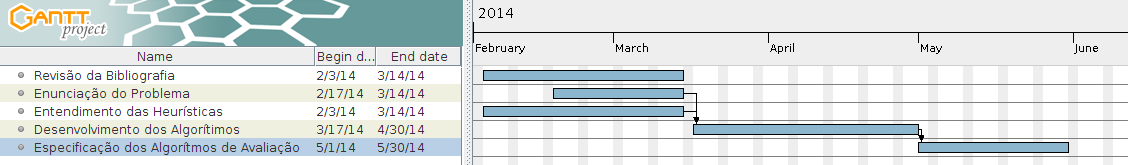
\includegraphics[width = 0.8 \linewidth]{imgs/cronograma}
      \caption{Cronograma de Atividades}
    \end{figure}
  \end{block}
}

%\chapter{Conclusão}
% TODO(depois): Fazer uma conclusão!


\chapter{Refer�ncias Bibliogr�ficas}

[1] CVETKOVIC, D. M., DOOB, M. e SACHS, H. Spectra of Graphs: Theory and
Application. Pure and Applied Mathematics: A Series of Monographs and Textbooks. Academic Press, New York, 1980.

[2] KIRKLAND, S.; NEUMANN, M.; SHADER, B.: Characteristic vertices of weighted trees via Perron values. Linear and Multilinear Algebra, Vol 40. 1996.

[3] http://dev.mysql.com/doc/refman/5.7/en/ acessado em 29 de stembro de 2013.

[4] http://www.neo4j.org/ acessado em 29 de setembro de 2013

[5] http://www.infoq.com/articles/graph-nosql-neo4j acessado em 29 de setembro de 2013

[6] http://www2.mat.ufrgs.br/~carvalho/pesquisa/interativa/graphenergy/graphspec.php

[7] RODRIGUES, S. "Sobre a conectividade alg�brica e seus autovetores na classe das �rvores". Disserta��o de Mestrado, Engenharia de Computa��o, SE8. Instituto Militar de Engenharia, 2013.

[8] SZWARCFITER, J. L. Grafos e Algoritmos Computacionais. Rio de Janeiro: Campus, 1984.


\newpage
$~$
\\

% Bibliografia no arquivo PRINCIPAL.bib



% Ap�ndices
%\input{Apendice.tex}

\end{document}
